\documentclass[conference]{IEEEtran}
\IEEEoverridecommandlockouts
% The preceding line is only needed to identify funding in the first footnote. If that is unneeded, please comment it out.
\usepackage{cite}
\usepackage{amsmath,amssymb,amsfonts}
\usepackage{algorithmic}
\usepackage{graphicx}
\usepackage{textcomp}
\usepackage{xcolor}
\def\BibTeX{{\rm B\kern-.05em{\sc i\kern-.025em b}\kern-.08em
    T\kern-.1667em\lower.7ex\hbox{E}\kern-.125emX}}
\begin{document}

\title{Decoding Factors in Altruistic Requests Leading to Success using Machine Learning and Natural Language Processing\\
}

\author{\IEEEauthorblockN{Siddhant Thakur}
\IEEEauthorblockA{\textit{Department of Data Science and Business Systems} \\
\textit{SRM Institute of Science and Technology}\\
Chennai, India \\
st7037@srmist.edu.in}
\and
\IEEEauthorblockN{M. Ramprasath}
\IEEEauthorblockA{\textit{Department of Data Science and Business Systems} \\
\textit{SRM Institute of Science and Technology}\\
Chennai, India \\
ramprasm@srmist.edu.in}
}

\maketitle

\begin{abstract}
Altruism is the definition of having a selfless concern for someone else’s well-being. Social media has now established a platform where people can be altruistic through different online philanthropic communities and question \& answer sites like Kickstarter or StackOverflow. Thousands and thousands of requests and questions are recorded on these sites, and people donate to or answer these pleas without considering their monetary benefit. An example of one of these online communities is the r/Random\_Acts\_Of\_Pizza subreddit on the popular social discussion forum Reddit. This subreddit is an online community where any user can post a request for a free pizza while stating the condition they are currently in, and the outcome of each request is either the user was successful or unsuccessful in getting a pizza. This paper attempts to understand the factors that lead to a request being successful or unsuccessful by proposing a new architecture of stacking two models, one dealing with the sparse vector generated from text and the other dealing with the dense features gathered by looking at previous works, in order to predict the success of a request. After implementing the architecture, we find that the probability estimated from the first model and the number of comments on the request post plays an essential role in predicting the outcome of a request.
\end{abstract}

\begin{IEEEkeywords}
Machine Learning, Natural Language Processing, Computational Social Science.
\end{IEEEkeywords}

\section{Introduction}
The amount of information shared in the form of text ever since the dawn of the internet has been appalling. In recent times, textual data has been one of the most important, if not the most important, sources of information. Efforts to get information out of text (or speech) have been underway since the 1950s when in the Georgetown-IBM Experiment, scientists successfully translated 60 Russian sentences into English and made some progress toward machine translation~\cite{gtown_exp}. Until the 1980s, the research work under Natural Language Processing was based on sets of hand-written rules, which became obsolete after the introduction of machine learning algorithms to textual data. The beginning of statistical NLP gave way to the advancement of many different subfields like machine translation, text classification, speech recognition, etc. Further, the need for state-of-the-art results in many natural language tasks gave rise to what is today known as Neural Natural Language Processing or Neural NLP~\cite{neural_nlp}. While utilizing deep learning methods, Neural NLP has become increasingly essential for sectors like healthcare and medicine.

Recently, a wave of use-cases in Computational Social Science has surfaced, requiring state-of-the-art NLP tools to solve them~\cite{compsci_nlp}. Be it determining biased news, identifying emotion behind tweets, or assessing the persuasiveness of an argument in a debate, the use of NLP tools for social causes has clearly increased. With the rise of social media and the use of Natural Language Processing in a social setting, the rise of philanthropic communities on the internet is notable. Websites like Kickstarter, Ketto, Reddit, and Kiva have made their presence immense and facilitated many people worldwide to get out of unpleasant situations via crowdfunding. For example, the Indian online crowdfunding platform, Ketto, has been responsible for raising over Rs. 2000 crores across 3.2 Lakh online fundraisers. This new era of online fundraising has undoubtedly helped people around the world and will certainly continue to do so. Our project focuses on a similar community forum, under the Reddit website, known as r/Random\_Acts\_Of\_Pizza~\cite{raop_paper}. The forum was created in the year 2010 with the aim of getting pizza to those who need it. Requesters could explain their situation in a post, giving information about why they need a pizza and how it would help them. It would then depend on the other users to donate a pizza to the requester.

The dataset used for this project was taken from the CS Stanford website, and the foundation for this project has been the work done by Althoff et al.~\cite{raop_base}. The dataset contains 5671 requests collected from the Reddit community between December 8, 2010, and September 29, 2013. There are 33 features present in the dataset, including a target variable containing the information about whether the requester received the pizza or not. The project proposes an architecture of a two-stack binary classification model to predict the success of an altruistic request. The first model deals with the textual data by utilizing textual feature extraction techniques to convert the raw text data into vector form and then classify the vector data against the target variable. The finished model is then used to estimate the probabilities of the request being successful by the text. This probability estimate is then used as a dense feature among other features, like account\_age of the requester, the number of upvotes and downvotes, etc., to predict the outcome of the request. We have then used the final model to determine the importance of each feature and how they contribute towards predicting the target variable.

\section{Literature Review}
In recent years, along with the increase in the research work under NLP in a social setting, there have been multiple attempts to decode linguistic factors in textual data and how they affect the success of requests. With the objective of interpreting what makes a favor successful, Althoff et al.~\cite{raop_base} discuss high-level social factors, like the status of the requester and the similarity between the requester and the donor, textual factors, like evidence of need and the sentiment of text, and, finally, temporal factors like age of the account and the time the request was made. A logistic regression model then binds these factors together to classify whether the request was successful or not. The model also allows the researchers to reason out the significance of independent variables in predicting the dependent variable. Similar to the base paper, Jacek and Sabrina et al.~\cite{raop_sent} focuses on the comparative analysis of different machine learning algorithms over the RAOP dataset. In addition to the social and linguistic factors, such as the requester's identity and how the requester is asking, the researchers also aim to extend the work by investigating the sentimental factors satisfying a donor.

H.-P. Hsieh et al.~\cite{raop_gprs} extend the base paper by introducing additional features like Topic, Role, and Centrality. These features handled the hidden meaning behind the text by using Bag of Words \& N-Gram and the role of interaction of the requester among other users. It then uses a novel model named the Graph-based Predictor for Request Success model (GPRS). It uses a Request Graph and Propagation-based Optimization algorithm to represent the feature similarity-based correlation between requests present in the data and learn the feature weights to compute probabilities of successful or unsuccessful requests, such that the requests having higher similarity scores will have the same label. Ahmed et al.~\cite{raop_gprs2} discuss the same method, focusing more on the Topic and Role as additional features.

Durmus and Cardie et al. 's~\cite{debate} work is based on debate.org, which provides a platform for people to express their opinions and beliefs. It takes on the task of judging which debater will be more successful. The paper provides a new dataset to study the effect of language use versus the prior beliefs on persuasion while proposing a controlled setting taking the political and religious ideology of the reader. It inculcates user-based features like ideology and opinion similarity and linguistic features like text length, sentiment, and features gathered using TF-IDF. Similarly, Yang et al.~\cite{neural_req1,neural_req2} also focus on modeling persuasive strategies using a semi-supervised hierarchical neural network incorporating both word-level and sentence-level attention to quantify persuasiveness.

\section{Proposed Architecture and Steps}
This project utilizes the crucial features gathered from the pre-existing dataset as well as the previous works in the literature review while framing our architecture consisting of a stack of two models to deal with the textual and numerical data separately. In this section, we will be stating the architecture developed and process followed in creating the two models.

\begin{figure}
\centering
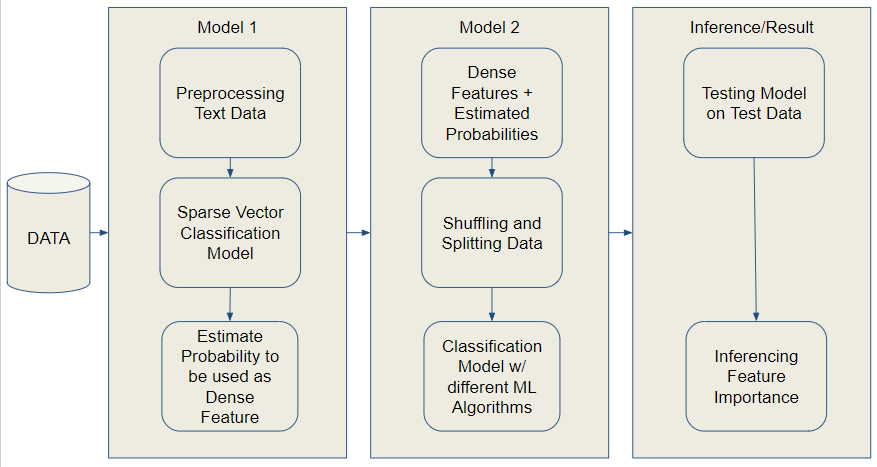
\includegraphics[width=\linewidth]{arch_diag.png}
\caption{Model Architecture} \label{fig1}
\end{figure}

\subsection{Data Exploration}
Data exploration allows for a better understanding of the dataset, making it easier for us to navigate the data better and select methods suitable for that data. After a simple exploration of the RAOP dataset, we notice that there are 5671 requests with an average success rate of 24.63\%, making it an imbalanced dataset. This will allow us to choose Stratified K-Fold instead of the standard K-Fold Cross Validation technique while training our models. Stratified K-Fold Cross Validation partitions the dataset so that the validation set will have an equal number of instances of the dependent variable~\cite{strat_kfold}. This ensures that no instance will overpower the other in the validation set.

\subsection{Text Preprocessing}
\paragraph{Lowercasing, Removal of Punctuation \& Stop-words}
are few of the most common preprocessing steps that allow us to reduce the redundancy between words. Similarly, Punctuation in a text can sometimes create difficulty in comprehending the text or extracting tokens. Therefore, it becomes necessary in some use cases to remove the punctuation in text.\\
Stop-words consist of the most common words used in any language and are usually removed from the text as they do not add any unique value to the text analysis. Therefore, we use the NLTK~\cite{nltk} list of English stop-words in our project to remove them from the request.
\paragraph{Regular Expression}~\cite{regex} has proven powerful in searching and manipulating text strings and has been an essential tool in text analytics. We can use it to find patterns in the text that we want to remove or edit. For example, in the project, we used the "re" python library to find and expand the contractions such as "don't," \& "can't," to "do not," \& "can not."
\paragraph{Tokenization} is the fundamental task of the NLP preprocessing pipeline in which we divide a piece of text into smaller units, and these units can be either words, subwords or characters. In this project, we have used the "regexp\_tokenize" function from the NLTK~\cite{nltk} library to tokenize the cleaned text.
\paragraph{Lemmatization} is the most crucial text preprocessing step that stems the word while ensuring it does not lose its meaning. The project uses of the Wordnet Lemmatizer present inside the NLTK~\cite{nltk} package. Wordnet~\cite{wordnet} is a large lexical database that aims to establish structured semantic relationships between words. We utilize the NLTK~\cite{nltk} interface of this database using the function lemmatize() of the instance WordNetLemmatizer().

\subsection{Feature Engineernig}
We split the numeric and textual data and separately work on it for the two different models.
\subsubsection{Numeric Data}
Based on the previous literature and knowledge, we manipulate the dataset in order to get the features. We use two features to understand how any posted request is doing in the community by subtracting the number of downvotes from the number of upvotes at retrieval as well as getting the number of comments at retrieval. We also add the length of the text as a feature to check if longer texts lead to the request being successful or not.\\
An "Evidence" feature is calculated by setting a value of 1 if there is a presence of any image link and 0 if there is no link present~\cite{raop_base}. For other features, we consider the account age of the requester and whether the requester has posted before in the RAOP subreddit. These features give us some information about the requester.
\subsubsection{Text Data}
We combine the title of the request and the main text of the request to get the final text which can then be converted into vectors using One-Hot Encoding~\cite{one_hot}, TF-IDF~\cite{tfidf}, Word2Vec~\cite{w2v}, and Doc2Vec~\cite{d2v} techniques.
\paragraph{One-Hot Encoding} or Count Vectorizing is the method of representing words by creating a vector having as many dimensions as the unique words in the vocabulary. Inside the vector, if the text data features that word, we put a “1” in that dimension; otherwise, we put “0”. This gives us a huge sparse vector representation of all the text requests in the data. However, one of the disadvantages of the Count Vectorizing technique is its inability to represent the semantic and statistical relationship between the data.
\paragraph{TF-IDF} vectors feature statistical representation of text regarding the word's importance or relevance in a document. This representation is constructive in information retrieval systems as it allows the system to look for more relevant words in the search query.
TF-IDF~\cite{tfidf} measure is the product of Term Frequency(TF)~\cite{tf} and Inverse Document Frequency(IDF)~\cite{idf}, where Term Frequency is a measure of the frequency of a word in a document, while Inverse Document Frequency is a measure of the importance of a word. Term Frequency can be defined as the ratio of a word's occurrence in a document to the total number of words present in a document. The IDF of a word is the natural log of the ratio of the total number of documents in the corpus to the number of documents containing that word. Therefore, it gives weightage to each word based on its frequency in the corpus.
\paragraph{Word2Vec} is another one of the frequently used embedding techniques which aim at learning embeddings for every word in the corpus such that the word vector in the embedding space best captures the meaning of the word~\cite{nlp_prac_book}. Word2Vec helps in capturing the semantic representation of the text. It uses neural networks to derive the word’s meaning from its context. Therefore, Word2Vec projects the meaning of the word in a high-dimensional vector space and clusters the word with similar meanings together. We used the pre-trained Word2Vec model over the Google News Corpus for this project~\cite{w2v}.\\
In order to find the sentence vector by using individual word vector representations, we calculate the average of the vectors of words in the text. Another method that has given good results in the past is calculating the minimum and maximum from the list of vectors of words in the text and concatenating it to form a more extensive vector representation~\cite{minmax}.
\paragraph{Doc2Vec}~\cite{d2v} is very similar to the Word2Vec~\cite{w2v} model in terms of its general architecture. In addition to learning the word vectors, it also learns the paragraph vector associated with the full text. There are two architectures of the Doc2Vec model called the Distributed Memory (DM) and the Distributed Bag of Words (DBOW). This project uses the Distributed Memory (DM) architecture of the Doc2Vec Model packaged under the Gensim library. 

\subsection{Modelling}
This section briefly describes the stack of two models present in our classification architecture. The architecture consists of two models, one that deals with the high-dimensional sparse vector converted from the textual data and the other model that deals with the dense features pre-existing in the dataset as well as the ones engineered by previous literature.
\subsubsection{Text Model}
The request title and the request text are combined with the target variable into a separate data frame. This data frame will be helpful in converting each row of the text data into a vector using different text embedding techniques mentioned in section 3.3. The resulting vectors from the different embedding techniques are then fed into different machine learning algorithms like Logistic Regression~\cite{lr}, Gaussian Naive Bayes~\cite{nb}, and Random Forest~\cite{rf}. (Note that we do not use K Nearest Neighbors~\cite{knn} or Support Vector Machines~\cite{svm} as they do not give a probability estimate needed for our second model.)\\
Based on the accuracy of the different models created by the combinations of different text embedding techniques and machine learning algorithms, we select the models to estimate the probability score for the success of the request and feed it to the final model.
\subsubsection{Final Model}
The final model consists of the numeric data present in the dataset, the derived features based on previous works, and the probability estimates of the text from the previously mentioned text models performing well. We use the Logistic Regression~\cite{lr}, Gaussian Naive Bayes~\cite{nb}, and Random Forest~\cite{rf} algorithms to create a classification model using the target variable of receiving a pizza as the dependent variable and the other dense features the independent variable. In order to ensure that the model will do well on unseen data and prevent overfitting, we also implemented a Stratified K-Fold cross-validation method~\cite{strat_kfold}.\\
The results of the following model are given under Section 4 with Accuracy~\cite{metrics}, Precision~\cite{metrics}, Recall~\cite{metrics}, and F1-Score~\cite{metrics} as the metrics.
\subsection{Parameter Optimization} 
Parameter Optimization or tuning is the name given to the process of selecting parameter values for a learning algorithm that leads to better performance of the algorithm. In this project, we decided to tune the hyperparameters of the Random Forest~\cite{rf} algorithm as there are a lot of parametric values that can affect the algorithm's performance. However, the parameters are not critical enough to need tuning for other algorithms, like Logistic Regression~\cite{lr} and Naive Bayes~\cite{nb}. This paper uses Randomized Search~\cite{rand_search} to optimize hyperparameters by randomly selecting points assigned inside a domain. Following this, Grid Search~\cite{rand_search} is applied to fine-tune the hyperparameters found by forming a grid of values based on the best values provided by the Randomized Search~\cite{rand_search}.
\subsection{Feature Importance}
Feature Importance is the technique of calculating a score for all the input features used in the model. This score refers to the importance of the variable in predicting the target variable.
We use the built-in Feature Importance technique in the Random Forest algorithm implemented in scikit-learn using Gini Importance~\cite{gini}. Gini Importance~\cite{gini} averages the decrease in node impurity for each feature over all trees in the ensemble to get the feature importance. We also use the SHAP~\cite{shap} interpretation to find the feature importances from the different models. In order to get this estimate of feature contribution to the prediction, it uses the Shapley ~\cite{shap} from game theory which helps us fairly distribute the contribution among the features. We apply both the methods to all the final models with the self-created dense features as well as the probability estimates from the text models.


\section{Results \& Inference}
There are three parts to be discussed in this section - performance of the text models, performance of the final model, and discussion of the importance of each feature in predicting the outcome. To measure the performance and understand the feature importance in the parts mentioned before, we decided to divide the dataset of 5671 into 4537 training rows and 1134 testing rows. This helps expose the classifier to train on the given data and measure its performance over the unseen data.
\subsection{Model Results}
\begin{figure}
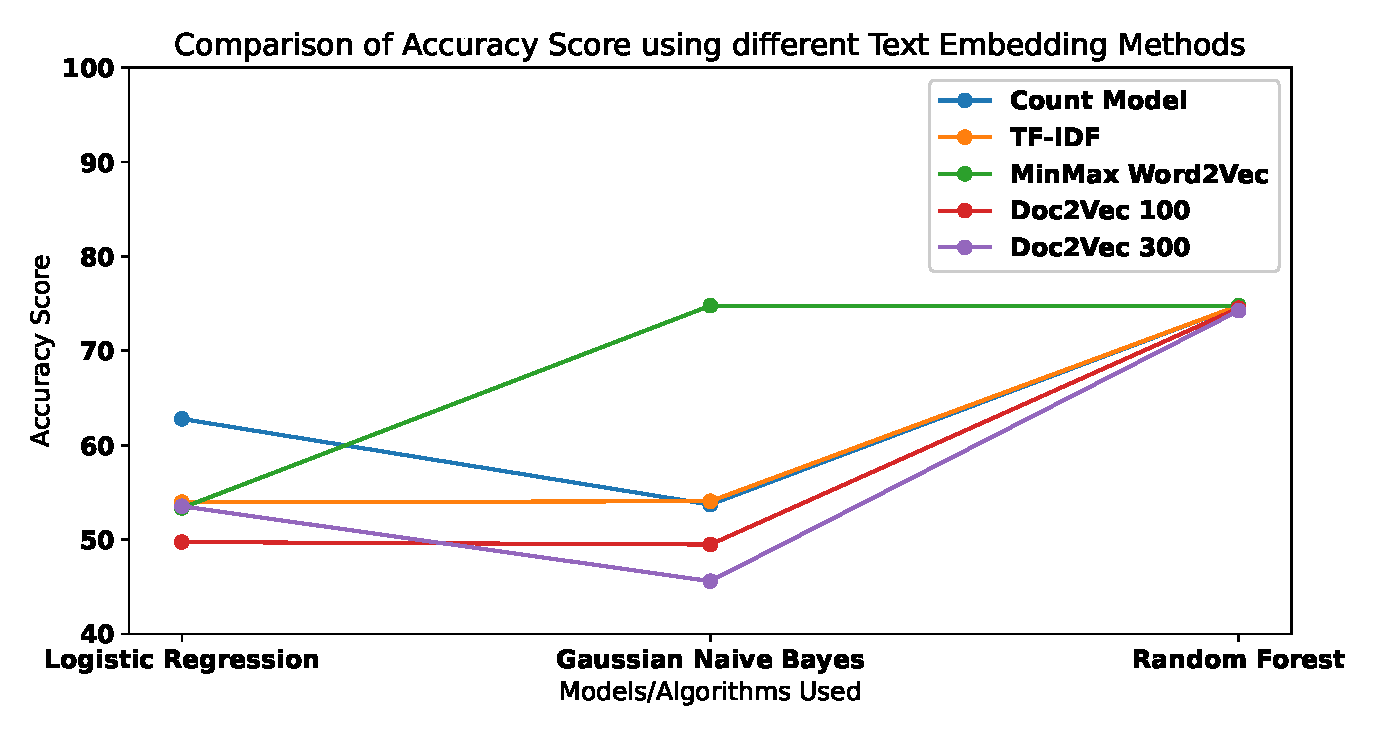
\includegraphics[width=\linewidth]{AccScoreTextModel.eps}
\caption{Comparison of Accuracy Score using different Text Embedding Methods} \label{fig2}
\end{figure}
For the performance of the text models, we can infer from the above plot, developed using matplotlib, that out of the three machine learning algorithms used, Random Forest~\cite{rf} performs equally well for each text embedding technique, while the performance under Logistic Regression~\cite{lr} improves with the use of a more complex and advanced text embedding technique. However, Gaussian Naive Bayes~\cite{nb} Classifier fails to achieve a reasonable threshold with any embedding techniques. Therefore, based on the inference from the graph, we choose the Random Forest version of all the embeddings.\\
Now to measure the performance of the final model, the test set separated from the primary data is first converted into vectors using the different embedding methods and then fed into the final model along with other numeric data. We make use of the metrics like Accuracy, Precision, Recall, and F-Score~\cite{metrics} in order to understand how the final model is performing on the test set.
\begin{figure}
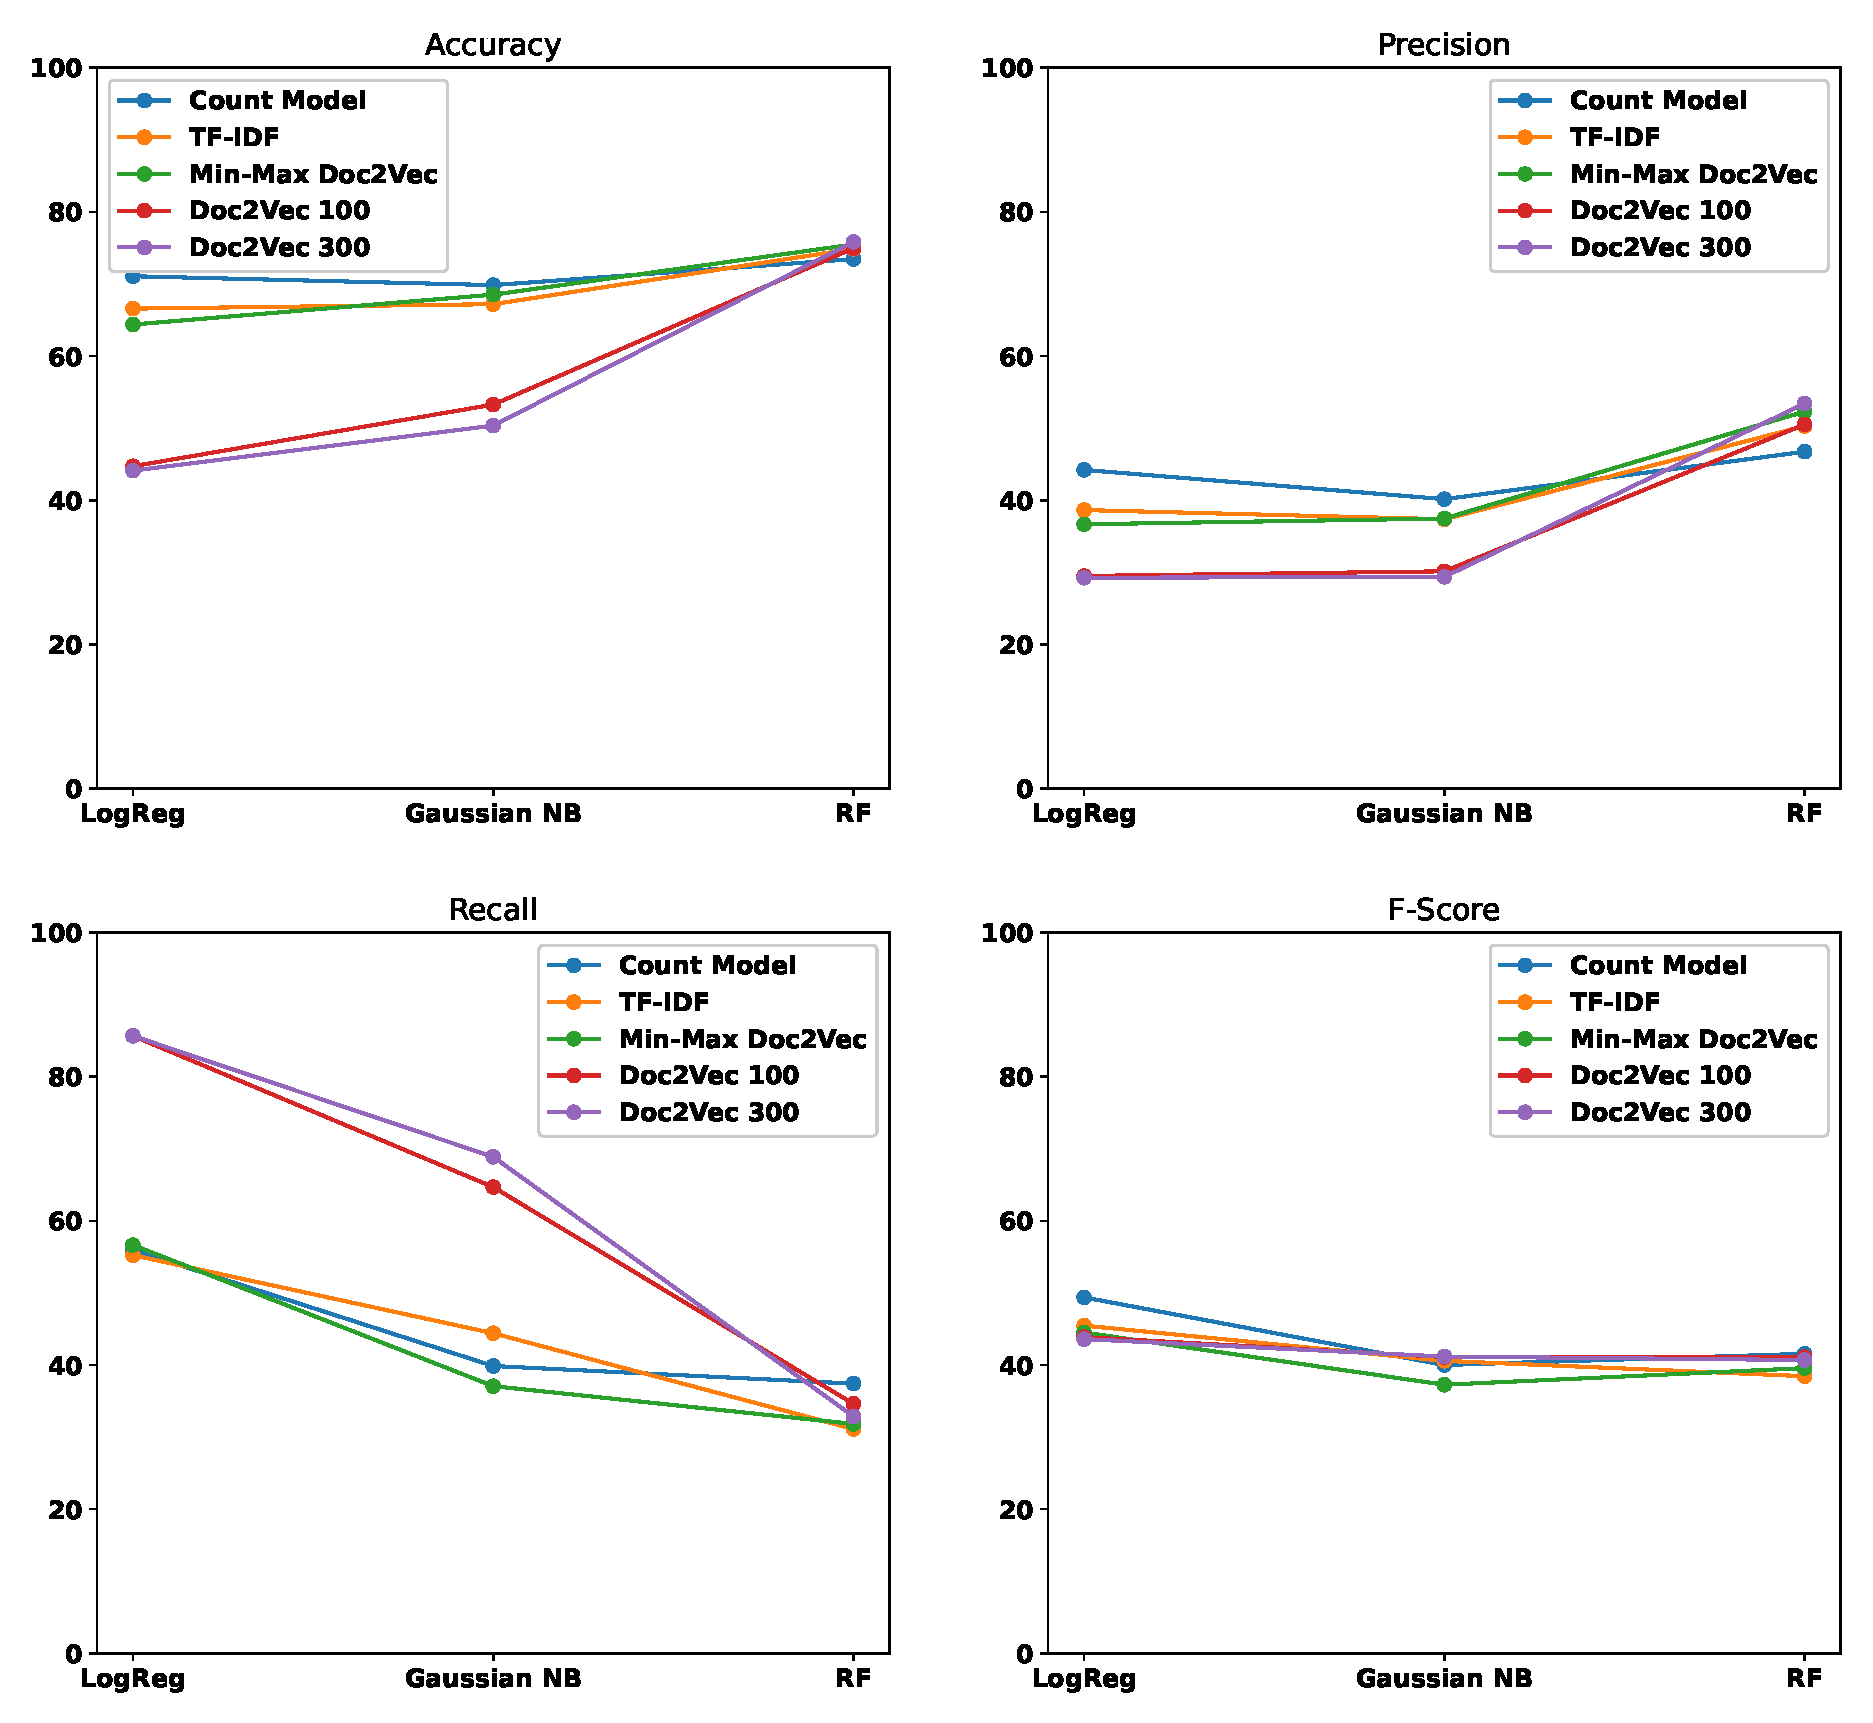
\includegraphics[width=\linewidth]{Final_Model_Performance.eps}
\caption{Performance of the Final Model in terms of Accuracy, Precision, Recall \& F-Score} \label{fig3}
\end{figure}
\\ The graph in Fig 3. shows the performance metrics of different machine learning algorithms applied over the original numeric data combined with the estimated probability received from the Random Forest versions of the embedded text data. We see that the model’s accuracy remains highest at around 75 when we use Random Forest to model the final data regardless of the embedding method used. However, for our use case, we are predicting whether a user will receive a pizza or not, which is a rare outcome with a chance of 24.63\%, according to our dataset. Therefore, we would also look at the measure of recall we are getting from the different models. From the graph, we infer that both the Doc2Vec embeddings, i.e., 100- and 300- dimensions, fed into a logistic model perform much better than other models in predicting the requesters that will receive a pizza. However, we also notice that the same models are less precise in predicting who actually receives the pizza and who does not.\\
On the other hand, the Logistic Model of the final data having Count and TF-IDF embeddings have a comparatively lower but appropriate recall score as well as a good precision score. Therefore, we attempt to get a balance between recall and precision by measuring the F-Score of the models. We see that, on average, all the models perform relatively close to each other in terms of F-score, with Logistic Regression version of Min-Max Word2Vec \& TF-IDF and Random Forest version of 300-dimension of Doc2Vec \& Min-Max Word2Vec have high F-scores. This suggests that the mentioned models maintain a good balance between precision and recall while predicting the outcome of a requester receiving a pizza or not.\\

\subsection{Model Inference}
In order to measure the importance of each feature, we use the SHAP~\cite{shap} values from the classifiers. The graph in Fig 4. provides the mean SHAP~\cite{shap} values of each feature utilized to predict the target variable. This mean-SHAP~\cite{shap} value refers to the impact of a feature on the model. Therefore, we see that the probability estimate generated from the text has a significant role in predicting whether a requester will receive their pizza or not. The number of comments on the request post, the upvotes minus downvotes, and the length of the text also have some part to play in predicting the outcome. However, from the models, we see that it hardly matters whether the requester has posted before in the subreddit or has attached an evidence link in the text as their SHAP~\cite{shap} values are very low.
\begin{figure}
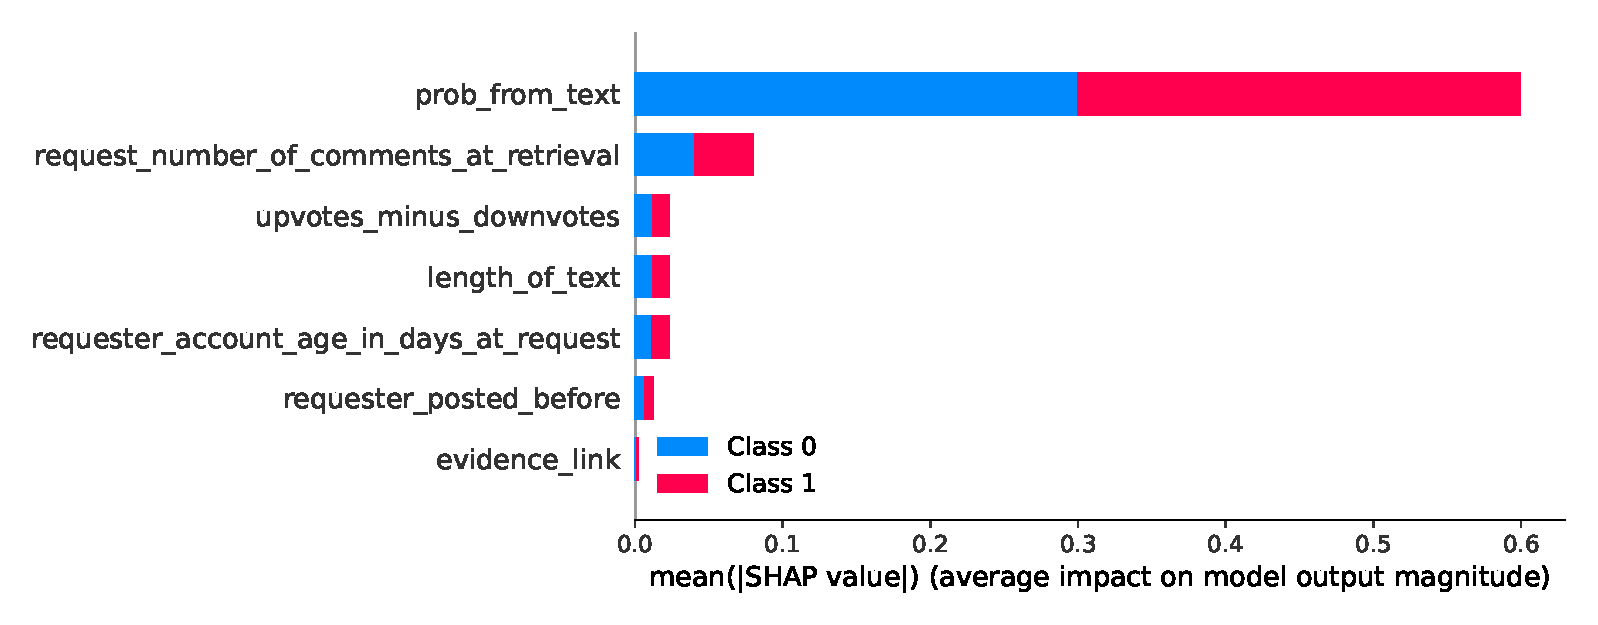
\includegraphics[width=\linewidth]{FeatureImportanceShapley_minmax.eps}
\caption{Ranking of Feature Importance in terms of SHAP values} \label{fig4}
\end{figure}

\section{Conclusion \& Future Work}
This work presents a stack of two models that separately deal with the text and numeric data. This allows us to reduce higher dimensional vectors generated from the text data to a probability estimate and retain the importance of the features present in the original dataset. The experimental findings validate the efficacy of our approach in terms of the performance metrics discussed in section 4. Therefore, given a requester posting a request, our model can predict whether it will stimulate any altruistic behavior from the other Redditors. Inferring the model also gives us an understanding of how useful other variables in the dataset were in predicting the outcome. In order to improve our work in the future, we can work around framing and combining different embedding techniques to get a vector representation of text, leading to better probability estimates and more satisfactory performance. Finally, this work can also be extended by using more sophisticated machine learning and deep learning models as well as adding more data in order to develop a more robust model.

\begin{thebibliography}{00}
\bibitem{gtown_exp}
Hutchins, W.J. (2004). The Georgetown-IBM Experiment Demonstrated in January 1954. In: Frederking, R.E., Taylor, K.B. (eds) Machine Translation: From Real Users to Research. AMTA 2004.

\bibitem{neural_nlp}
Tom Young, Devamanyu Hazarika, Soujanya Poria, Erik Cambria (2017). Recent Trends in Deep Learning Based Natural Language Processing. arXiv:1708.02709.

\bibitem{compsci_nlp}
Bamman, D., Doğruöz, A. S., Eisenstein, J., Hovy, D., Jurgens, D., O’Connor, B., … Volkova (2016). Proceedings of the First Workshop on NLP and Computational Social Science.

\bibitem{raop_paper}
Althoff, T., Salehi, N., Nguyen, T. (2013). Random Acts of Pizza : Success Factors of Online Requests.

\bibitem{raop_base}
Althoff, T., Salehi, N., Nguyen, T. (2013). Random Acts of Pizza : Success Factors of Online Requests.

\bibitem{raop_sent}
J. Filipczuk, E. Pesce \& S. Senatore, Sentiment detection for predicting altruistic behaviors in Social Web: A case study, 2016 IEEE International Conference on Systems, Man, and Cybernetics (SMC), 2016.

\bibitem{raop_gprs}
Hsieh, Hsun-Ping, Yan, Rui, Li, Cheng-Te. (2016). Will I Win Your Favor? Predicting the Success of Altruistic Requests. Pacific-Asia Conference on Knowledge Discovery and Data Mining.

\bibitem{raop_gprs2}
Ahmad, Amreen \& Ahmad, Tanvir & Bhatt, Abhishek. (2019). A Novel Approach for Predicting the Outcome of Request in RAOP Dataset. Proceedings of GUCON 2018.

\bibitem{debate}
Esin Durmus \& Claire Cardie. 2018. Exploring the Role of Prior Beliefs for Argument Persuasion. In Proceedings of the 2018 Conference of the North American.

\bibitem{neural_req1}
Diyi Yang, Jiaao Chen, Zichao Yang, Dan Jurafsky, and Eduard Hovy. 2019. Let’s Make Your Request More Persuasive: Modeling Persuasive Strategies via Semi-Supervised Neural Nets on Crowdfunding Platforms. In Proceedings of the 2019 Conference of the North American Chapter of the Association for Computational Linguistics: Human Language Technologies.

\bibitem{neural_req2}
Chen, J., \& Yang, D. (2021). Weakly-Supervised Hierarchical Models for Predicting Persuasive Strategies in Good-faith Textual Requests. AAAI.

\bibitem{strat_kfold}
Raschka, S. (2018). Model Evaluation, Model Selection, and Algorithm Selection in Machine Learning. CoRR, arXiv:1811.12808.

\bibitem{nltk}
Loper, Edward \& Bird, Steven. (2002). NLTK: the Natural Language Toolkit. CoRR, arXiv:cs/0205028

\bibitem{regex}
Erwig, Martin \& Gopinath, Rahul. (2012). Explanations for Regular Expressions.

\bibitem{wordnet}
Fellbaum, C.D. (2000). WordNet : an electronic lexical database. Language, 76, 706.

\bibitem{one_hot}
Harris, David \& Harris, Sarah. (2007). Digital Design and Computer Architecture. 

\bibitem{tfidf}
Manning, C., Raghavan, P., \& Schütze, H. (2008). Introduction to Information Retrieval. Cambridge: Cambridge University Press.

\bibitem{w2v}
Mikolov, T., Chen, K., Corrado, G., \& Dean, J. (2013). “Efficient Estimation of Word Representations in Vector Space.” arXiv:1301.3781.

\bibitem{d2v}
Le, Q. V., \& Mikolov, T. (2014). Distributed Representations of Sentences and Documents.

\bibitem{tf}
H. P. Luhn, A Statistical Approach to Mechanized Encoding and Searching of Literary Information, in IBM Journal of Research and Development.

\bibitem{idf}
SPARCK JONES, K. (1972), A Statistical Interpretation of Term Specificity and its Application in Retrieval, Journal of Documentation.

\bibitem{nlp_prac_book}
Sowmya Vajjala, Bodhisattwa Majumder, Anuj Gupta, Harshit Surana (2020). Practical Natural Language Processing: A Comprehensive Guide to Building Real-World NLP Systems.

\bibitem{minmax}
Boom, C. D., Van Canneyt, S., Demeester, T., \& Dhoedt, B. (2016). “Representation learning for very short texts using weighted word embedding aggregation.” Pattern Recognition Letters, 80, 150–156.

\bibitem{lr}
Cramer, J.S., The Origins of Logistic Regression (December 2002). Tinbergen Institute Working Paper No. 2002-119/4

\bibitem{nb}
Rish, Irina. (2001). An Empirical Study of the Naïve Bayes Classifier. IJCAI 2001 Work Empir Methods Artif Intell. 3.

\bibitem{rf}
Breiman, L. Random Forests. Machine Learning 45, 5–32 (2001).

\bibitem{knn}
Cunningham, Padraig \& Delany, Sarah. (2007). k-Nearest neighbour classifiers. Mult Classif Syst. 

\bibitem{svm}
Evgeniou, Theodoros \& Pontil, Massimiliano. (2001). Support Vector Machines: Theory and Applications.

\bibitem{metrics}
Goutte, Cyril \& Gaussier, Eric. (2005). A Probabilistic Interpretation of Precision, Recall and F-Score, with Implication for Evaluation. Lecture Notes in Computer Science.

\bibitem{rand_search}
James Bergstra, Yoshua Bengio. (2012). Random Search for Hyper-Parameter Optimization.

\bibitem{gini}
Menze, Bjoern \& Kelm, Bernd \& Masuch, Ralf \& Himmelreich, Uwe \& Bachert, Peter \& Petrich, Wolfgang & Hamprecht, Fred. (2009). A comparison of Random Forest and its Gini importance with standard chemometric methods for the feature selection and classification of spectral data.

\bibitem{shap}
Lundberg, S., \& Lee, S.-I. (2017). A Unified Approach to Interpreting Model Predictions. arXiv:1705.07874

\end{thebibliography}
\end{document}
